\chapter{Introdução}
\label{cha:introducao}

O intercâmbio de informações é um tema chave da logística moderna. Este nicho é chamado de logística da informação e lida com o fluxo de informações entre humanos e/ou máquinas dentro ou entre organizações \cite{haftor2011information}, que se agrupam formando uma rede de criação de valor por meio de informações.

Com o cenário de comércio em um mundo intrinsecamente globalizado, as Cadeias de Suprimentos (CS) e suas interdependências tornam-se mais complexas \cite{surana2005supplychain}. O compartilhamento de informações entre os elos da CS, portanto, torna-se uma forma de trazer mais eficiência ao seu funcionamento como um todo.

Quando se trata de informações relativas a um produto, o conceito de Memória Digital do Produto (MDP) pode ser utilizado como forma de coletar, armazenar e fornecer informações. A MDP se refere a sistemas que permitem a coleta de dados em todas as fases do ciclo de vida do produto para distribuição e/ou análise \cite{wahlster2007digitalmemory}. Os dados de interesse do produto se relacionam a qualquer fase de sua CS, o que abrange dados de produção, montagem, distribuição (transporte) \cite{brandherm2011productmemory}, bem como padrões de uso pelo cliente final, etc.

O compartilhamento destas informações, geradas a partir de dados, favorece o desenvolvimento de novas versões do próprio produto e funciona também como um elo permanente entre o fornecedor e o cliente no pós-venda \cite{brandherm2011productmemory}, permitindo que o produto mantenha atualizações e quaisquer outras melhorias instantaneamente.

Tais conceitos se encaixam com a Indústria 4.0 (I4.0), que tem como fundamentos a inserção de novas tecnologias com o propósito de oferecer um alto nível de automação e intercâmbio de informações entre equipamentos e produtos \cite{lasi2014industryfour}.

Portanto, surge na I4.0 oportunidades para a criação de novas soluções centradas na transparência das informações pela CS \cite{lasi2014industryfour} proporcionada pelo compartilhamento, além de novas metodologias para a extração e análise dessas informações para desenvolvimento de outros produtos aperfeiçoados.

A Logística da Informação e a MDP, mencionadas anteriormente, são intrinsecamente relacionados à I4.0, que por sua vez faz o uso extensivo de conhecimentos e técnicas das áreas de Gestão da Informação (GI) e Tecnologia de Informação e Comunicação (TIC).

A I4.0 surgiu a partir da crescente integração das TICs com os processos industriais, criando as bases para uma revolução industrial \cite{hermann2016design}. As modificações em relação às tecnologias de manufatura proporcionam um alto nível de automação e intercâmbio de informações entre equipamentos, produtos e demais atores em um ambiente de manufatura \cite{lasi2014industryfour}.

O nome I4.0 se dá ao fato de ser considerada a quarta revolução com relação às tecnologias de produção industrial, sendo as ``revoluções industriais'' consideradas evoluções tecnológicas que levaram a mudanças significativas na forma de produção da época. Tal histórico de revoluções no campo da indústria é ilustrado na \autoref{fig:i4}.

\begin{figure}[htb]
	\centering
	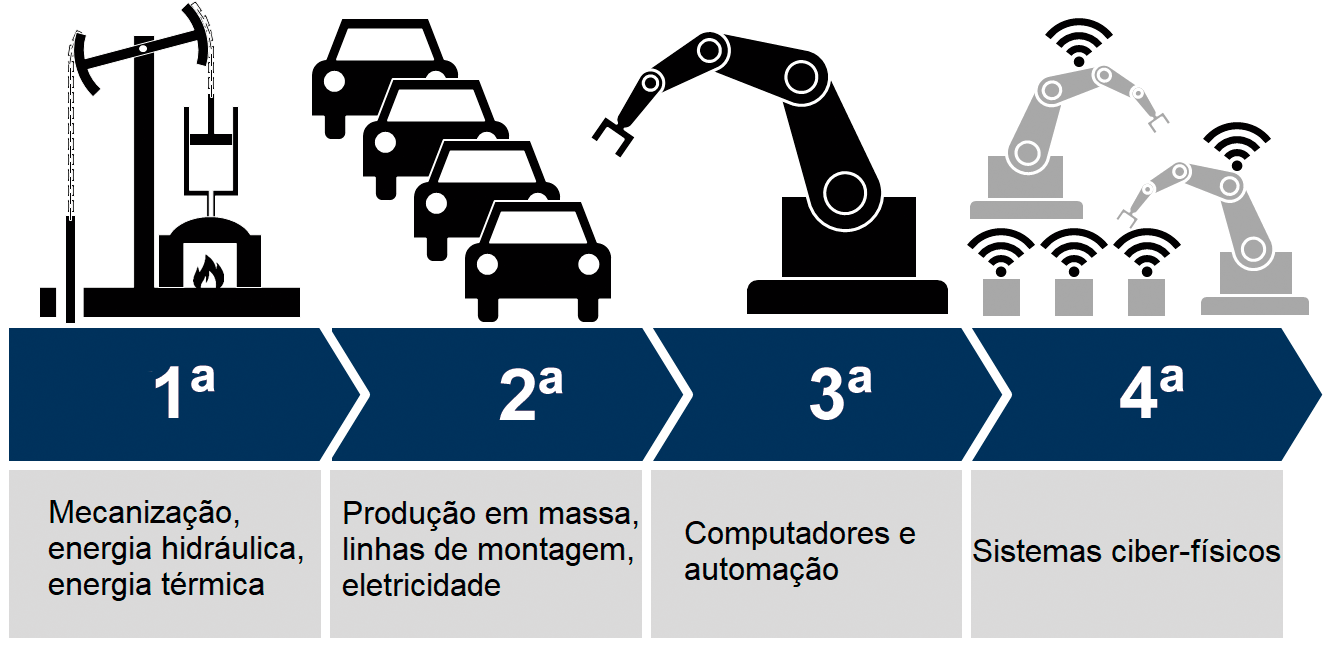
\includegraphics[width=1\textwidth]{i4.png}
	\caption{As revoluções industriais.}
	\label{fig:i4}
	\fonte{\citeonline{lasi2014industryfour} (adaptado).}
\end{figure}

Tais modificações são essenciais devido às novas necessidades da própria indústria e às mudanças de padrões de consumo do mercado. Isto acarreta transformações no cenário operacional. Algumas das causas dessas mudanças operacionais são \cite{lasi2014industryfour}:

\begin{itemize}

	\item Períodos de desenvolvimento curtos: Os períodos de desenvolvimento e inovação de produtos estão sendo reduzidos. A alta capacidade de inovação está se tornando um fator de sucesso para muitas empresas (\textit{Time to market});

	\item Individualização sob demanda: Os compradores passam a definir as condições de compra. Essa tendência leva a uma crescente individualização de produtos com características altamente personalizadas e, em casos extremos, a produtos individuais;

	\item Flexibilidade: Devido à individualização sob demanda, novas estruturas e organizações na indústria são essenciais para a fabricação de produtos com alto grau de personalização. É necessária uma maior flexibilidade no desenvolvimento do produto, especialmente na produção;

	\item Descentralização: Para lidar com condições específicas de cada demanda, são necessários procedimentos mais rápidos de tomada de decisão. Para isso, as hierarquias organizacionais precisam ser reduzidas, dando ao produto maior independência sobre seu próprio processo de fabricação;

	\item Eficiência de recursos: A maior eficiência sobre o uso dos recursos sempre é algo desejável, porém sua importância se intensifica com as tendências de aumento dos preços dos recursos, bem como a mudança social no contexto de aspectos ecológicos. Isto exige um foco mais intensivo em sustentabilidade, o que decorre em uma maior racionalidade (ou eficiência) na utilização dos recursos.

\end{itemize}

\citeonline{hermann2016design} elencam alguns princípios da I4.0 que devem ser considerados para o projeto de soluções, sendo eles: interoperabilidade, transparência de informação, descentralização de decisões e assistência técnica.

Estes princípios são diretrizes para o desenvolvimento de arquiteturas de sistemas para a I4.0. As arquiteturas surgem com a necessidade de se definir padrões para a implantação de um sistema. Por ser um assunto novo, as arquiteturas de sistemas produtivos voltadas para a quarta revolução industrial também se encontram em estágio inicial \cite{pisching2018arquitetura}. Um dos principais modelos de arquitetura para a I4.0 é o RAMI4.0 (Modelo de Arquitetura de Referência para a Indústria 4.0) \cite{hankel2015rami}. Esse modelo de arquitetura foi apresentado na feira industrial de Hanôver na Alemanha em abril de 2015.

Assim como o RAMI4.0, outros modelos de arquitetura para a I4.0 trazem propostas similares, como é o caso do IMSA (\textit{Intelligent Manufacturing System Architecture}), IIRA (\textit{Industrial Internet Reference Architecture}) e IVRA (\textit{Industrial Value Chain Reference Architecture}) \cite{li2018architectures}. Porém, o RAMI4.0 é uma proposta mais abrangente e flexível em relação às novas tecnologias \cite{hankel2015rami}.

O RAMI4.0 é uma representação tridimensional dos aspectos de uma indústria moderna, conforme a \autoref{fig:rami4}.

\begin{figure}[htb]
	\centering
	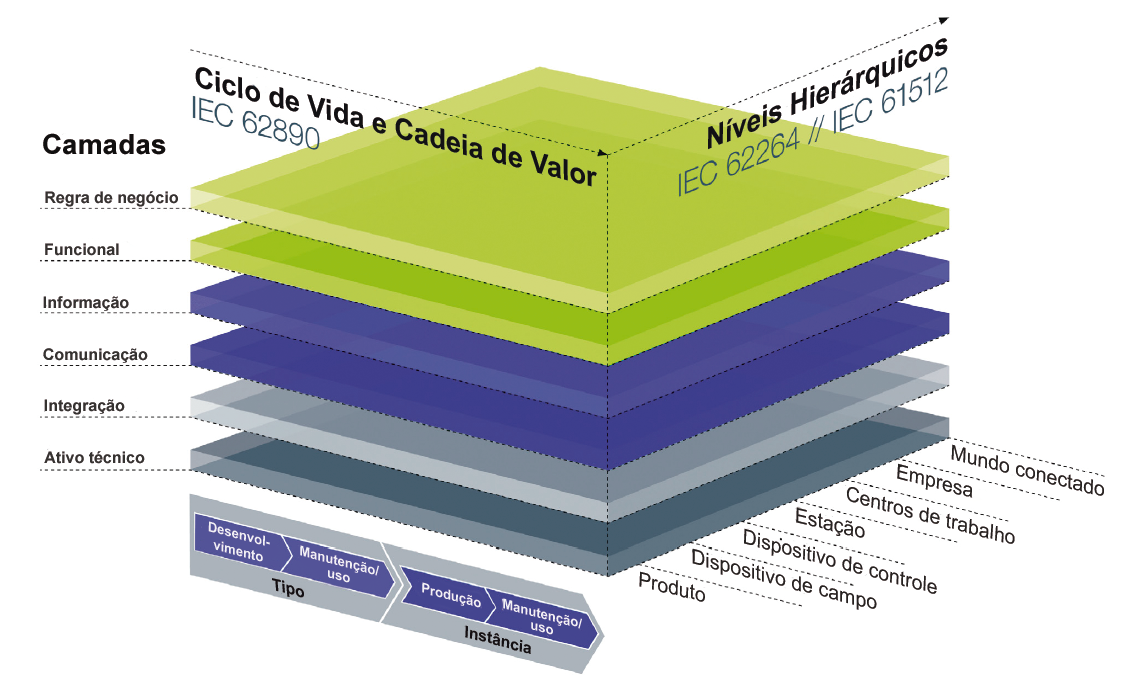
\includegraphics[width=1\textwidth]{rami4.png}
	\caption{Representação do RAMI4.0.}
	\label{fig:rami4}
	\fonte{\citeonline{adolphs2015rami} (adaptado).}
\end{figure}

Alguns dos conceitos introduzidos pelo RAMI4.0 são \cite{bader2019aas}:

\begin{itemize}
	\item Componente 4.0 (C4.0): junção de um ativo físico com sua parte digital;
	\item Submodelo: representações de informações de um determinado ativo, incluindo suas características, propriedades, condições, parâmetros, dados de medições e capacidades.
\end{itemize}

O RAMI4.0, como o próprio nome diz, é um modelo de arquitetura. Isto significa que é um modelo a ser utilizado para a elaboração de outras arquiteturas e, desta forma, define as bases para a elaboração de arquiteturas de sistemas que sejam interoperáveis entre si.

\section{Motivação}
\label{sec:motivacao}

Os conceitos de I4.0 e MDP surgiram em 2011 \cite{kagermann2011industrie} e 2007 \cite{wahlster2007digitalmemory}, respectivamente. A área multidisciplinar de estudo envolvendo MDP e I4.0 surgiu em 2013 com o projeto SemProM \cite{wahlster2013semprom}, porém ainda quando I4.0 era um tema abrangente sem diretrizes concretas para a sua implementação, o que ocorreria em 2013 por meio do documento de recomendações para implementação da iniciativa estratégica ``Industrie 4.0'' \cite{kagermann2013recommendations}, antes da criação do RAMI4.0, que seria divulgado em 2015 por um periódico alemão \cite{hankel2015rami}.

Alguns estudos como \citeonline{lasi2014industryfour} citam MDP como oportunidade de estudo e aplicação dentro da I4.0. Outros como \citeonline{weyer2015standardization} e \citeonline{paelke2014augmented} implementaram sistemas envolvendo ambos os conceitos, porém sem considerações sobre CS.

Há estudos na área multidisciplinar de I4.0 e MDP, principalmente no meio acadêmico, empresarial e governamental alemão pelo fato de esses conceitos terem surgido na Alemanha. Porém nenhum trabalho até o presente momento relaciona o RAMI4.0 com a MDP. I4.0 e a MDP são temas correlacionados, porém ainda não devidamente abordados em conjunto na literatura, o que aponta uma lacuna de conhecimento dentro de I4.0 a ser explorada.

Estudos sobre o RAMI4.0 são importantes no sentido de padronizar a implementação da I4.0 em empresas de diferentes negócios, garantindo assim a interoperabilidade dos serviços. Integrar a MDP ao RAMI4.0 enriquece o nível de discussão sobre essa arquitetura de referência visando uma futura adoção generalizada por parte de empresas por todo o mundo.

A ``Plattform Industrie 4.0'' é uma das principais redes mundiais de discussão sobre I4.0 \cite{kagermann2013recommendations, acatech2014plattform, hartmut2019plattform}. O Conselho de Pesquisa da Plattform Industrie 4.0 é o comitê consultivo estratégico da Plattform Industrie 4.0 e identifica necessidades de pesquisa e ações em torno da I4.0. O comitê identificou e definiu quatro temas-chave de abordagens no setor tecnológico, econômico, metodológico e social/legal para se implementar com sucesso a I4.0 \cite{hirsch-kreinsen2019keythemes}, conforme mostrado na \autoref{fig:keythemes-i4}. Isso significa que os tópicos elencados são temas com alto potencial de otimização de rotinas e processos de produção existentes no cenário de I4.0.

\begin{figure}[htb]
	\centering
	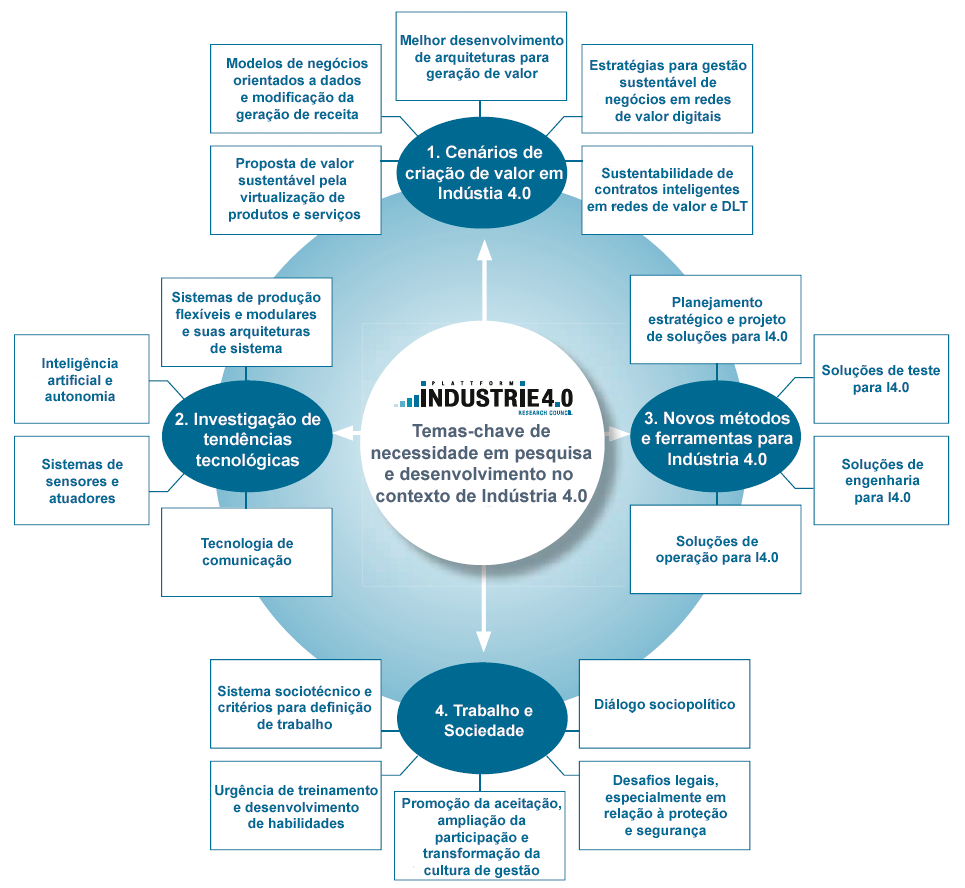
\includegraphics[width=1\textwidth]{keythemes-i4.png}
	\caption{Temas-chave de pesquisa e desenvolvimento em I4.0.}
	\label{fig:keythemes-i4}
	\fonte{\citeonline{hirsch-kreinsen2019keythemes} (adaptado).}
\end{figure}

Dentre os temas elencados na \autoref{fig:keythemes-i4}, destacam-se os subitens relacionados ao tópico ``Cenários de criação de valor em Indústria 4.0'' por estarem altamente relacionados ao RAMI4.0 e à geração de valor por meio da MDP. Estes são temas de grande oportunidade dentro do cenário de I4.0, especialmente se considerados os métodos de análise de dados já estabelecidos.

\section{Objetivos}
\label{sec:objetivos}

Dadas as motivações do trabalho apresentadas na \autoref{sec:motivacao}, o objetivo deste trabalho é a elaboração de uma arquitetura baseada no RAMI4.0 para o compartilhamento da MDP ao longo da CS.

Para se alcançar o objetivo geral, este é desmembrado em metas, representadas pelos objetivos específicos, que são:

\begin{itemize}
	\item \textbf{Integração da MDP ao C4.0} (\autoref{sec:estrutura-aas}): a MDP é incorporada ao C4.0 do produto para que assim esteja disponível para consulta pelos membros da CS na I4.0;
	\item \textbf{Levantamento de submodelos do produto e suas propriedades} (\autoref{sec:submodelos-produto}): as informações a serem compartilhadas pela CS devem estar encapsuladas em forma de submodelos e propriedades a fim de se adequarem ao RAMI4.0. Aqui são identificadas e classificadas as informações relevantes do produto de interesse aos membros da CS;
	\item \textbf{Levantamento dos impactos em geração de valor com o compartilhamento da MDP} (\autoref{sec:geracao-de-valor}): as informações possuem potencial de geração de valor ao produto e ao negócio. Aqui são apontados estes impactos e como eles ocorrem durante o ciclo de vida do produto;
	\item \textbf{Detalhamento dos elementos da arquitetura} (\autoref{sec:componentes-e-operacoes}): os componentes e operações principais da arquitetura são detalhados;
	\item \textbf{Descrição do processo de compartilhamento de informações} (\autoref{sec:fluxo-de-fornecimento-de-servicos}): o fluxo das informações utilizando a arquitetura é analisado considerando a CS completa com todos os membros principais em cenários realísticos;
	\item \textbf{Mapeamento das operações para as camadas do RAMI4.0} (\autoref{sec:mapeamento-das-operacoes}): a arquitetura é analisada com relação à interação entre cada par de C4.0 em cada camada do RAMI4.0;
\end{itemize}

\section{Estrutura do trabalho}
\label{sec:estrutura}

O capítulo de introdução (\autoref{cha:introducao}) apresenta uma abordagem inicial dos conceitos que são tratados ao longo do trabalho, a motivação e objetivos da pesquisa.

O \autoref{cha:fundamentos} apresenta a revisão bibliográfica com a fundamentação dos conceitos necessários para o desenvolvimento da arquitetura.

O \autoref{cha:ciclo-de-vida} apresenta a proposta de integração da MDP ao C4.0 para a interoperabilidade dentro da I4.0.

O \autoref{cha:arquitetura} apresenta a arquitetura proposta para o compartilhamento da MDP baseada no RAMI4.0.

Finalmente, no \autoref{cha:conclusao} são feitas as considerações sobre a pesquisa com comentários sobre os resultados alcançados e trabalhos futuros.
